\documentclass{report}
\usepackage[T1]{fontenc} % Fontes T1
\usepackage[utf8]{inputenc} % Input UTF8
\usepackage[backend=biber, style=ieee]{biblatex} % para usar bibliografia
\usepackage{csquotes}
\usepackage[portuguese]{babel} %Usar língua portuguesa
\usepackage{blindtext} % Gerar texto automaticamente
\usepackage[printonlyused]{acronym}
\usepackage{hyperref} % para autoref
\usepackage{graphicx}

\bibliography{bibliografia}


\begin{document}
%%
% Definições
%
\def\titulo{Relatório Guess Number}
\def\data{Maio de 2021}
\def\autores{João Pedro Raposo Ferreira, Maria João Vieira Pinto}
\def\autorescontactos{(103625) joaop.ferreira@ua.pt, (103482) mariajvpinto@ua.pt}
\def\versao{VERSAO}
\def\departamento{DETI}
\def\empresa{Universidade de Aveiro}
\def\logotipo{ua.pdf}
%
%%%%%% CAPA %%%%%%
%
\renewcommand{\contentsname}{Índice}
\begin{titlepage}

\begin{center}
%
\vspace*{50mm}
%
{\Huge \titulo}\\ 
%
\vspace{10mm}
%
{\Large \empresa}\\
%
\vspace{10mm}
%
{\LARGE \autores}\\ 
%
\vspace{30mm}
%
\begin{figure}[h]
\center
\includegraphics{\logotipo}
\end{figure}
%
\vspace{30mm}
\end{center}
%
\begin{flushright}
\versao
\end{flushright}
\end{titlepage}

%%  Página de Título %%
\title{%
{\Huge\textbf{\titulo}}\\
{\Large \departamento\\ \empresa}
}
%
\author{%
    \autores \\
    \autorescontactos
}
%
\date{\data}
%
\maketitle

\pagenumbering{roman}

%%%%%% RESUMO %%%%%%
\begin{abstract}
Este relatório irá abordar a maneira como o projeto AP2 foi efuatuado, mais especificamente descrever o que nos motivou, a sua implentação, tanto do mesmo bem como do seu algoritmo, a realização de alguns testes que comprovam o bom funcionamento do código e, por fim, uma breve análise dos resultados obtidos.
\end{abstract}

%%%%%% Agradecimentos %%%%%%
% Segundo glisc deveria aparecer após conclusão...
%\renewcommand{\abstractname}{Agradecimentos}
%\begin{abstract}
%Eventuais agradecimentos.
%Comentar bloco caso não existam agradecimentos a fazer.
%\end{abstract}


\tableofcontents
% \listoftables     % descomentar se necessário
% \listoffigures    % descomentar se necessário


%%%%%%%%%%%%%%%%%%%%%%%%%%%%%%%
\clearpage
\pagenumbering{arabic}

%%%%%%%%%%%%%%%%%%%%%%%%%%%%%%%%
\chapter{Introdução}
\label{chap.introducao}

Este trabalho consistiu na criação de um jogo onde o utilizador(client) tinha que tentar adivinhar o número secreto gerado pelo servidor. Durante o jogo, o cliente tem várias tentativas para adivinhar este número secreto, assim como pode desistir, ainda que o jogo não tenha chegado ao fim. O jogo termina quando o número de tentativas chega ao fim ou quando o jogador acerta no valor do número secreto. As operações efetuadas pelo jogador são passadas ao programa através de um conjunto de instruções que o servidor reconhece. 
Ao longo de várias tentativas fomos fazendo e aperfeiçoando o nosso código para que o jogo funcione o melhor possível.

Este documento está dividido em três capítulos. Depois desta pequena  introdução, no
Capítulo 2 serão apresentados os passos efetuados para o desenvolvimento do trabalho. Já Capítulo 3 são apresentados os resultados obtidos ao longo do código e, finalmente,
no último capítulo são apresentadas as conclusões do trabalho realizado.


\chapter{Desenvolvimento}
\label{chap.metodologia}
Este jogo foi desenvolvido para que fosse "jogado" através de um terminal.

Os dois ficheiros principais deste projeto são o "server.py" que é o servidor que recebe as instruções em formato de dicionários do cliente, que se refere ao ficheiro client.py, e que, a partir destes consegues executar enumeras funções.

As funções que estão na base deste jogo são a "START", "GUESS", "QUIT" e "STOP".

A primeira funcionalidade (Figura 2.1) é a verificação do utilizador, ou seja, é verificado se o utilizador já se encontra registado ou não.
%%%%
\vspace{10mm}
    \begin{figure}[h]
        \begin{center}
            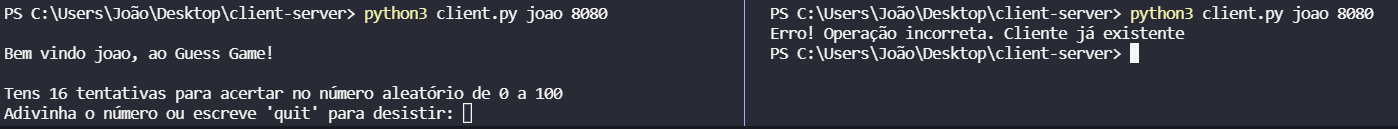
\includegraphics[scale=0.5]{outro.png}
            \caption{Erro de cliente existente}
        \end{center}
    \end{figure}


\pagebreak

Depois disso começa realmente o jogo (Figura 2.2). É concedido um número aleatório de tentativas e é da responsabilidade do "client" assegurar que o que é introduzido no terminal corresponde ao que é pedido, caso contrário é mostrada um pequeno aviso sendo possível ao utilizador refazer a sua ação e continuar o jogo (Figura 2.3).

\vspace{10mm}
    \begin{figure}[h]
        \begin{center}
            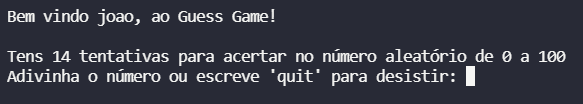
\includegraphics[scale=0.5]{unknown.png}
            \caption{Inicio do jogo}
        \end{center}
    \end{figure}
    
\vspace{10mm}
    \begin{figure}[h]
        \begin{center}
            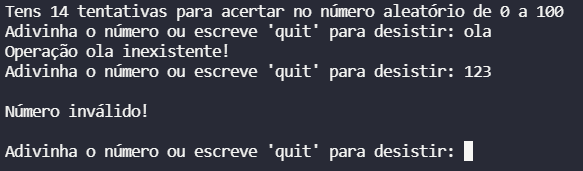
\includegraphics[scale=0.5]{unknown (1).png}
            \caption{Inputs inválidos}
        \end{center}
    \end{figure}
\pagebreak

Este código foi feito de maneira robusta e com o objetivo de prevenir qualquer erro, propositado ou não, efetuado pelo utilizador. Quer isto dizer que apenas existem duas formas de terminar o jogo. Uma delas é esgotando o número de tentativas ou encontrando o número secreto e a outra é apenas digitar a palavra "quit" (Figura 2.4) que é recebida pelo "client" e enviada em forma de dicionário para o "server" onde este se encarrega de atualizar o ficheiro "report.csv" (Figura 2.5) com os dados do utilizador, enquanto o "client" encerra o programa.

\vspace{10mm}
    \begin{figure}[h]
        \begin{center}
            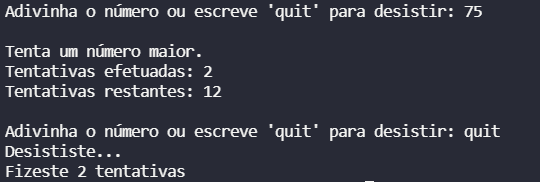
\includegraphics[scale=0.5]{unknown (3).png}
            \caption{Saída do programa}
        \end{center}
    \end{figure}

\vspace{10mm}
    \begin{figure}[h]
        \begin{center}
            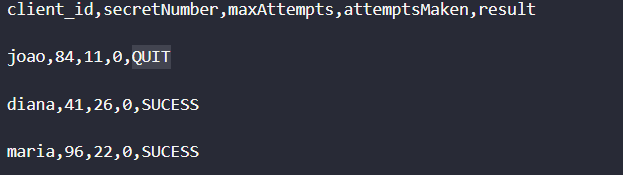
\includegraphics[scale=0.5]{unknown (2).png}
            \caption{Atualização dos dados}
        \end{center}
    \end{figure}

Como se pode ver pela imagem (Figura 2.5), o ficheiro "report.csv" tem como objetivo registar os dados do utilizador (nome, número secreto, jogadas efetuadas, e a maneira como o jogo foi terminado).


\chapter{Resultados}
\label{chap.resultados}
Como se pode concluir pelas imagens e pelo que foi escrito, achamos que conseguimos ao máximo evitar qualquer tipo de input inválido que pudesse impedir o normal funcionamento do programa. 

\chapter*{Contribuições dos autores}
Elaboramos este trabalho com um grande esforço de ambas as partes, ou seja, a nosso ver achamos que ambos contribuímos de igual modo para a realização deste projeto.


%%%%%%%%%%%%%%%%%%%%%%%%%%%%%%%%%
%\chapter*{Acrónimos}
%\begin{acronym}
%\acro{ua}[UA]{Universidade de Aveiro}
%\acro{miect}[MIECT]{Mestrado Integrado em Engenharia de Computadores e Telemática}
%\acro{lei}[LEI]{Licenciatura em Engenharia Informática}
%\acro{glisc}[GLISC]{Grey Literature International Steering Committee}
%\acro{deti}[DETI]{Departamento de Electrónica, Telecomunicações e Informática}
%\end{acronym}


%%%%%%%%%%%%%%%%%%%%%%%%%%%%%%%%%

\end{document}